\part{Les objectifs de ce projet}
    
    {\large
    L'objet de ce mémoire est de présenter si et comment le machine learning pourrait appuyer le Groupe Pomona dans la gestion des informations produit qu'il commercialise.
    Le groupe et sa gestion de l'information produit sont présentés en annexe \mref{business}.
    }

    \chapter{Les cas d'usage}
    \label{use_cases}

        \section{Objectifs : Qualité et productivité}

        La gestion de l'information produit est un processus lourd, avec des étapes de contrôle redondantes visant à assurer la qualité de la donnée (cf. annexe \mref{controles}), en particulier la cohérence des informations transmises avec le contenu des pièces jointes mises à disposition.
        Un traitement automatique des documents mis à disposition permettrait de décharger les personnes qui interviennent dans le processus (fournisseurs, acheteurs, gestionnaires de référentiels, ingénieurs qualité) et de garantir une meilleure pertinence de l'information produit.

        \section{La préalimentation d'information}
        Une des manières de gagner en productivité et en qualité serait :
        \begin{itemize}
            \item de modifier l'interface homme machine de l'écran de saisie des données par le fournisseur, pour que le chargement des pièces jointes se fasse en premier
            \item d'interpréter le contenu des pièces jointes dès qu'elles sont chargées, pour alimenter les autres champs de saisie
            \item laisser ensuite au fournisseur la possibilité de compléter et corriger ces informations avant de les soumettre à Pomona
        \end{itemize} 
        Il est illusoire d'automatiser totalement la saisie et d'imaginer se passer d'une saisie complémentaire par le fournisseur.
        La mise en place de la GDSN (cf. section \mref{GDSN}), qui permet pourtant de faire transiter par EDI les données produit de manière standardisée et efficace, n'a pas permis de s'affranchir de cette tâche.
        Sous réserve d'avoir un outil suffisamment fiable, on pourrait faire gagner du temps aux fournisseurs et améliorer la qualité de l'information produit.
        Néanmoins, plusieurs freins existent à la mise en place 
        \begin{itemize}
            \item cela n'a d'intérêt que si le système est capable de produire de l'information structurée avec une fiabilité élevée (par exemple, 80\% de données correctes serait un minimum)
            \item cela entre en concurrence directe avec le système GDSN - avec la question de la manière de gérer les conflits entre les information issues de ce réseau et celles extraites des pièces jointes
            \item cela apporte l'essentiel de la valeur aux fournisseurs, et pas au groupe
        \end{itemize}

        \section{Le contrôle des informations transmises}

        Plus le taux de détection des erreurs est élevé, et plus les erreurs sont détectées tôt, mieux c'est : 
        \begin{itemize}
            \item la qualité des données s'en trouve évidemment améliorée
            \item le processus est plus court en temps, en évitant les aller-retours
            \item on décharge l'ensemble des acteurs, en limitant le nombre d'interventions de chacun, ainsi que la charge administrative de synchronisation de leurs actions             
        \end{itemize}
        Les différentes étapes possibles pour lesquelles effectuer un contrôle sont présentées à la \reffig{fig:processus_article_aide_ctrle}.

        \begin{figure}[htbp]
            \begin{center}
            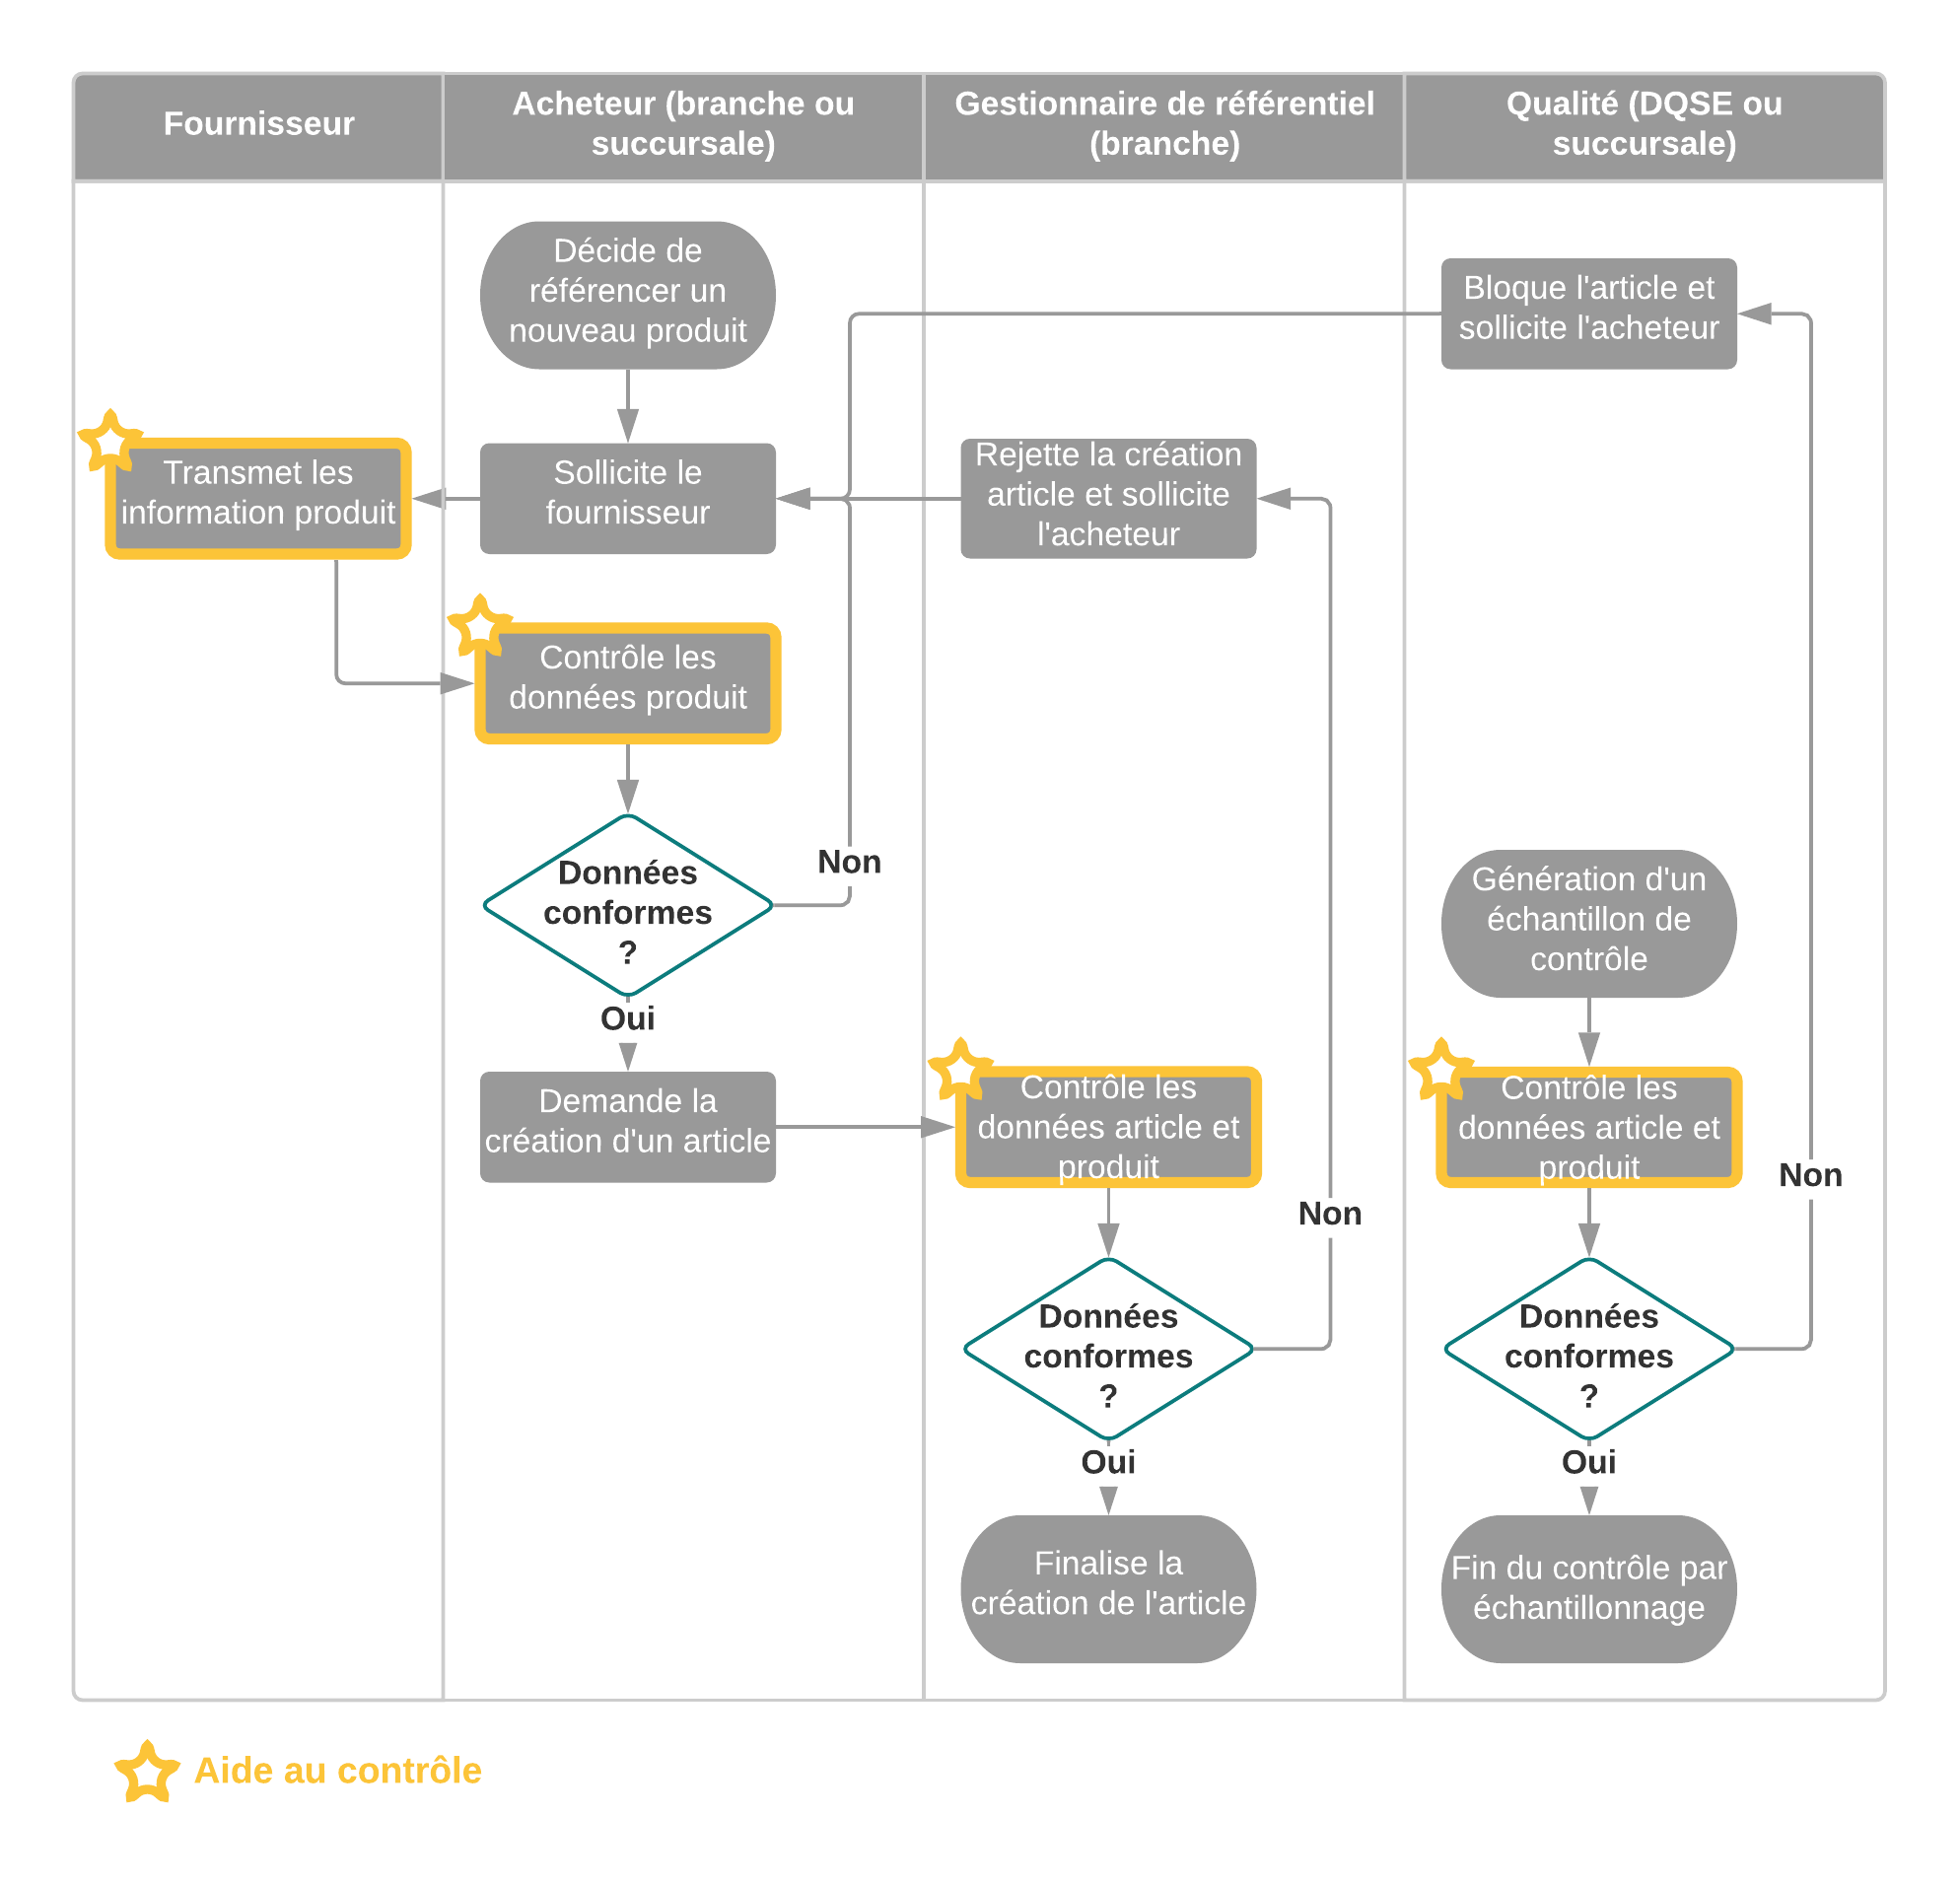
\includegraphics[width=0.9\linewidth]{img/Processus_de_creation_article_avec_aide_au_controle.png}
            \end{center}
            \caption{\'{E}tapes du processus article pouvant être améliorées}
            \label{fig:processus_article_aide_ctrle}
        \end{figure}    

            \subsection{Le contrôle à la saisie fournisseur}
            Si on déclenche un contrôle au moment où le fournisseur soumet les données et qu'on l'alerte en cas d'incohérence, on peut dès le début du processus éviter une erreur.
            L'avantage d'avoir une identification des problèmes aussi tôt est qu'on économise immédiatement au moins une étape de contrôle des données.

            \subsection{L'aide aux vérifications Pomona}
            Lors des contrôles inclus au sein du processus, on pourrait mettre en évidence les incohérences détectées entre pièces jointes et données à contrôler.
            Cela permettrait de fiabiliser les étapes de contrôle, et éviter qu'une erreur soit détectée tardivement (par les gestionnaires de référentiel ou les ingénieurs qualité).
            C'est d'autant plus intéressant que la première étape de contrôle est faite par les acheteurs.
            Dans la mesure où c'est une tâche administrative qui n'est pas dans leur c{\oe}ur de métier, elle est souvent effectuée rapidement et est peu efficace.

            \subsection{Les contrôles en masse asynchrones}
            Enfin, il pourrait être pertinent de faire tourner de manière asynchrone des contrôles de qualité de données sur l'ensemble de la base.
            Il pourrait sembler inutile d'effectuer cette tâche alors qu'on a une validation des données par l'application (contrôles \og informatiques \fg) et par des contrôleurs humains.
            Néanmoins, il arrive fréquemment que des changements de règles de gestion informatiques ou métier soit mis en place, sans que les données soient ensuite remises à jour.
            Par exemple, les mentions des traces d'allergènes dans les ingrédients était par le passé retirées des listes d'ingrédients, alors qu'elle sont aujourd'hui incluses. 
            Mais aucun chantier de remise à niveau de l'historique n'a été entrepris au moment du changement de règle, d'où des données qui ne sont pas alignées avec les règles de gestion.


    \chapter{Présentation rapide des données relatives au cas d'usage}

        \section{Les listes d'ingrédients}
        \label{listes_ingredients}

        Une information produit dont l'exactitude est critique sont les listes d'ingrédients.
        La construction des listes d'ingrédients doit suivre les règles suivantes, même si l'application n'est pas toujours parfaitement respectée :
        \begin{itemize}
            \item elle doit détailler l'ensemble des ingrédients, y compris les additifs et les arômes
            \item elle doit être triée par ordre d'importance pondérale décroissante (i.e. les ingrédients les plus représentatifs en poids doivent être cités en premier)
            \item la quantité de certains ingrédients (en pourcentage de la masse) par exemple ceux mis en valeur sur l'étiquetage ou dans la dénomination de vente (ex. gâteau aux fraises, pizza au jambon)
        \end{itemize}
        Même s'il ne s'agit pas d'une exigence réglementaire, le Groupe Pomona demande à ses fournisseurs de ne pas distinguer les ingrédients par phase comme cela se fait parfois.
        Cela signifie, par exemple, séparer une partie de la composition du produit (la pâte de la garniture pour une tarte, la sauce et les raviolis, \dots).
        De telles pratiques peuvent parfois induire le consommateur en erreur, comme par exemple dans la liste d'ingrédients suivante (s'applique à des chips de légumes):
        \begin{quotation}
            Légumes 64\% (betterave, panais, carottes, patates douces), huile de tournesol, sel marin.
        \end{quotation}
        Sans l'artifice d'avoir regroupé les légumes en une seule phase, le premier ingrédient de la liste aurait pu être l'huile de tournesol, qui est un ingrédient moins attractif pour un consommateur de chips de légumes.

        Quelques exemples de listes d'ingrédients sont présentées à la \reftable{tbl:exemple_ingred}.

        {\renewcommand{\arraystretch}{2}%
        \begin{table}[htbp]
            {\scriptsize
            \begin{center}%
            \begin{tabular}{p{5cm}l}
\toprule
                                        Désignation produit fournisseur &                                                                                                                                                                                              Liste d'ingrédients \\
\midrule
                                            HARICOTS BLANCS À LA TOMATE &                                                                                                                        Haricots blancs (UE et non UE), eau, sel, tomate concentré, antioxydant : acide citrique. \\
                                                 POIVRE VERT DÉSHYDRATÉ &                                                                                                                                                                                                 100\% poivre vert \\
            Crème de marron de l'Ardèche en boîte 500 g CLEMENT FAUGIER &                                                                                                                        Châtaignes 50\%, sucre, marrons glacés, sirop de glucose, eau, extrait naturel de vanille  \\
 Velouté de poireaux pommes de terre hyposodé en sachet 800 g NEFF MADA &  Pomme de terre 32 \%, amidon modifié de pomme de terre, fécule de pomme de terre, maltodextrine de blé, poireau 8 \%, arômes naturels, sucre, oignon, antiagglomérant : E551 "nano", plantes aromatiques, curcuma \\
                         Poivre Kampot rouge en pot 50 g TERRE EXOTIQUE &                                                                                                                                                                                      Poivre de Kampot rouge 100\% \\
\bottomrule
\end{tabular}
%
            \caption{Exemples de listes d'ingrédients}%
            \label{tbl:exemple_ingred}%
            \end{center}%
            }
        \end{table}
        }

        \emphbox{
        Les contraintes ci-dessus s'appliquant aux listes d'ingrédients font qu'en général, il s'agit d'une énumération d'ingrédients, sans doublon.
        }


        \section{Pièces jointes}
            \label{pieces_jointes}

            Dans le PIM, les pièces jointes - intéressantes au titre de l'information produit - gérées au niveau du produit sont les suivantes :
            \begin{itemize}
                \item les fiches techniques fournisseur
                \item les étiquettes produits
            \end{itemize}
    
            D'autres types de pièces jointes sont gérées, mais elle ne seront pas décrites dans le détail (car non pertinente pour le cas d'usage présenté):
            \begin{description}
                \item[les certificats des labels : ] ce sont des documents pdf produits par les organismes de certification attestant qu'un produit peut porter un label. Ils sont mis à disposition par les fournisseurs
                \item[les images produit : ] ce sont des visuels des produits (photographies ou images construites) qui visent à être utilisées dans des catalogues ou sur les sites de vente en ligne
                \item[les fiches logistiques : ] ce sont des fichiers qui viennent compléter les informations de la fiche technique lorsque cette dernière ne porte pas les informations relatives à la hiérarchie logistique. 
                \item[les fiches techniques et argumentaires Pomona : ] ce sont des documents pdf produits par le PIM, stockées sur les articles, qui reprennent des informations produit et article (cf. section \mref{produit_article}). Elles sont transmises aux clients ou utilisés par les commerciaux Pomona.
                Elles permettent d'avoir une présentation uniforme de l'ensemble de l'assortiment (les fiches techniques fournisseur ont des formats très variables)
            \end{description}

            \subsection{Fiches techniques fournisseur}
            \label{fiches_techniques}

                \subsubsection{Généralités sur les fiches techniques}
            Une fiche technique fournisseur est un document, d'une à une dizaine de pages, qui reprend l'essentiel des informations techniques à propos du produit.
            Elles portent globalement l'ensemble des informations produit telles que présentées à la section \mref{info_produit}.
            C'est le document le plus complet vis-à-vis des informations produit, il porte en général des informations complémentaires à toutes les informations présentes sur l'emballage du produit (les étiquettes).
            En général, une fiche technique ne porte d'information que pour un unique produit, mais dans le cas d'assortiments, les informations peuvent être relatives à plusieurs d'entre eux. Cf. la fiche technique pour l'assortiment de confitures, présentée en annexe \mref{ex:FT_confiture}.
            Les fiches techniques fournisseur sont des pièces jointes qui sont collectées par la branche \'{E}piSaveurs depuis la mise en place du logiciel de gestion historique GIP (cf. section \mref{GIP}), et il s'agit d'une données obligatoire dans le PIM également.
            
                \subsubsection{Le format des fiches techniques}
            Dans le PIM, ces pièces jointes sont collectées et stockées sous forme de pdf (les autres formats de fichier ne sont pas autorisés).
            Sauf de rares exceptions, il s'agit de fichiers issus de logiciels de traitement de texte, au format A4 portrait.
            Ce sont des documents techniques, et sont donc en général très structurés, avec des paragraphes, sous-paragraphes, tableaux, \dots
            Comme cela se constate aisément sur les exemples présentés en annexe, même si les informations portées sont sensiblement toujours les mêmes, les formats de ces documents sont extrêmement variables.
            Il n'y a aucun standard réglementaire ou normatif relatif à la construction de ces fiches, chaque industriel constitue donc son propre format.
            On a donc un foisonnement de formats différents.

                \subsubsection{Focus sur le mode de présentation de quelques informations}
            Les informations produits sont en général présentées de la manière suivantes dans les fiches techniques :
            \begin{description}
                \item[Liste d'ingrédients : ] elle est quasiment toujours présentée sous forme de texte (identique à la liste d'ingrédients telle qu'affichée sur l'emballage du produit), mais elle peut également être présentée sous forme de tableau. Cf. la fiche technique présentée en annexe \mref{ex:FT_poivron} (celle-ci ne porte pas de liste d'ingrédients sous forme de texte)
                \item[Allergènes : ] il peuvent être :
                \begin{itemize}
                    \item soit mis en évidence dans la liste d'ingrédients via la police (gras, souligné, majuscules)
                    \item soit listés hors de la liste d'ingrédient, sous forme de texte. Cf. la fiche technique présentée en annexe \mref{ex:FT_pannacotta}
                    \item soit listés sous forme d'un tableau reprenant l'ensemble des allergènes réglementaires, et le niveau de présence associé (présence, contamination croisée ou absence). Cf. la fiche technique présentée en annexe \mref{ex:FT_ciboulette}
                \end{itemize}
                \item[Données nutritionnelles : ] les données nutritionnelles sont en général présentées sous forme de tableau dans les fiches techniques. De plus, les informations nutritionnelles sont souvent données pour 100 grammes (ou 100 millilitres), ce qui est réglementaire, mais également parfois pour une portion. La taille de la portion est définie arbitrairement par le fournisseur.
                Cf. la fiche technique de la préparation pour panna cotta \mref{ex:FT_pannacotta}.
                \item[Données logistiques : ] les informations relatives à la hiérarchie logistiques se présentent souvent sous forme de tableaux.
                L'interprétation de ces tableaux est généralement complexe et nécessite un peu de réflexion.
            \end{description}
            
            \subsection{\'{E}tiquettes produit}
            \label{etiquettes_produit}

            \subsubsection{Généralités sur les étiquettes}
            L'étiquette produit est la partie de l'emballage du produit qui porte les informations produit.
            Selon la technologie de l'emballage - très liée au fait que le produit est plutôt brut ou plutôt transformé - il peut s'agir :
            \begin{itemize}
                \item d'une photo de l'étiquette collante apposée sur l'extérieur de l'emballage du produit (cf. exemple des étiquettes de lentilles \mref{ex:ET_lentilles} ou de sauce soja \mref{ex:ET_saucesoja})
                \item d'un applat de l'emballage, ou son bon-à-tirer, qui est le document qui est ensuite envoyé aux chaînes de production pour impression (cf. exemple du bon à tirer pour la préparation pour panna cotta \mref{ex:ET_pannacotta})
                \item ou de tout autre visuel montrant une partie indissociable de l'emballage physique du produit (ex : un photo de la face de l'emballage qui porte les inforations produit, cf. l'étiquette des madeleines \mref{ex:ET_madeleine})
            \end{itemize}
            Pour résumer, l'étiquette est une pièce jointe qui représente l'information produit qui \og voyage avec le produit \fg.
            La cohérence entre les données de l'étiquette et l'information produit transmises aux client est un enjeu majeur, dans la mesure où ce sont en général les informations portées par le produit physique qui sont correctes.
            La collecte systématique des étiquettes produit est une nouveauté arrivée avec la mise en place du PIM pour \'{E}piSaveurs (mai 2019).
            En théorie, les étiquettes mises à disposition par les fournisseurs devraient systématiquement porter les informations réglementaires.
            Or, du fait de la relative nouveauté de cette collecte, les pièces jointes transmises ne sont pas toujours conformes (cf. l'étiquette des lentilles \mref{ex:ET_lentilles}, qui ne portent aucune information nutritionnelle ou de composition).

            \subsubsection{Le format des étiquettes}
            Comme les fiches techniques, ces pièces jointes sont collectées et stockées sous forme de pdf (les autres formats de fichier ne sont pas autorisés).
            Du fait que les natures mêmes de ces pièces jointes sont diverses (cf. paragraphe précédent), il n'existe pas de format prédominant.

            \subsubsection{Focus sur le mode de présentation de quelques informations}
            Les étiquettes portent moins d'information que les fiches techniques.
            Par exemple, elles ne portent pas d'information sur la hiérarchie logistique, les données administratives (tel que le taux de TVA ou la nomenclature douanière), les codes d'identification (hormis le GTIN qui est présent sur le code à barre), \dots
            Les durées de vie ne sont pas mentionnées : sur l'emballage d'un produit seule la date limite apparaît, et elle dépend du lot de production.
            En règle générale, hormis quelques allégations volontairement affichées par l'industriel, l'étiquette ne porte que les informations réglementaires.
            Les information produit positionnées sur l'étiquette se présentes de la manière suivante :
            \begin{description}
                \item[Liste d'ingrédients : ] elle est toujours présentée sous forme d'un texte énumérant les ingrédients (cf. la section \mref{listes_ingredients} qui détaille le contenu d'une liste d'ingrédients)
                \item[Allergènes : ] ils sont uniquement mis en évidence dans la liste d'ingrédients, par l'utilisation d'une police spécifique (gras, souligné, majuscule, \dots). Cela peut se constater par exemple sur l'étiquette de madeleines \mref{ex:ET_madeleine} ou celle de la sauce soja \mref{ex:ET_saucesoja}
                \item[Données nutritionnelles : ] les données nutritionnelles se présentent souvent sous forme d'un tableau, toujours avec les valeurs pour 100 grammes ou 100 millilitres, et parfois pour une portion.
                Il peut arriver, plutôt pour les produits peu transformés, que ces données soient simplement écrite sous forme de texte tel que \begin{quote}\'{E}nergie : 1101 kJ/260 kcal, Glucides : 57 g, Sucres : 52 g, Protéines : 4,3 g, Sel : 7,1 g\end{quote} 
            \end{description}           

        \section{Récapitulatif de la complétude des données}

            Dans cette section, les indicateurs présentés se basent sur les notions \og En qualité \fg et \og Hors qualité \fg, qui sont explicitées en annexe \mref{statuts}. 

            \subsection{Complétude des listes d'ingrédients}



            \subsection{Complétude des pièces jointes}

            Si on analyse le niveau de renseignement des données pour les étiquettes et les fiches techniques, on obtient la \reftable{tbl:attached_files_counts}.

            %{\renewcommand{\arraystretch}{1.5}%
            \begin{table}[htbp]
                \begin{center}
                {\tiny
                \begin{tabular}{|l|ccc|ccc|ccc|ccc|ccc|ccc|}
\toprule
{} & \multicolumn{6}{c|}{En qualité} & \multicolumn{6}{c|}{Hors qualité} & \multicolumn{6}{c|}{Total} \\
{} & \multicolumn{3}{c}{Fiche technique} & \multicolumn{3}{c|}{Etiquette} & \multicolumn{3}{c}{Fiche technique} & \multicolumn{3}{c|}{Etiquette} & \multicolumn{3}{c}{Fiche technique} & \multicolumn{3}{c|}{Etiquette} \\
{} &             cpt &  sur &    \% &       cpt &  sur &    \% &             cpt &  sur &   \% &       cpt &  sur &   \% &             cpt &   sur &   \% &       cpt &   sur &   \% \\
\midrule
\textbf{Epicerie} &            3007 & 3007 & 100\% &      2996 & 3007 &  99\% &            4791 & 5755 & 83\% &      1921 & 5755 & 33\% &            7798 &  8762 & 88\% &      4917 &  8762 & 56\% \\
\textbf{Boissons} &             355 &  355 & 100\% &       352 &  355 &  99\% &             458 &  551 & 83\% &       184 &  551 & 33\% &             813 &   906 & 89\% &       536 &   906 & 59\% \\
\textbf{Alcools } &             253 &  253 & 100\% &       253 &  253 & 100\% &             296 &  354 & 83\% &        74 &  354 & 20\% &             549 &   607 & 90\% &       327 &   607 & 53\% \\
\textbf{Hygiène } &             768 &  768 & 100\% &       688 &  768 &  89\% &            1509 & 1733 & 87\% &       420 & 1733 & 24\% &            2277 &  2501 & 91\% &      1108 &  2501 & 44\% \\
\textbf{Chimie  } &             130 &  130 & 100\% &       130 &  130 & 100\% &             310 &  329 & 94\% &       127 &  329 & 38\% &             440 &   459 & 95\% &       257 &   459 & 55\% \\
\textbf{Total   } &            4513 & 4513 & 100\% &      4419 & 4513 &  97\% &            7364 & 8722 & 84\% &      2726 & 8722 & 31\% &           11877 & 13235 & 89\% &      7145 & 13235 & 53\% \\
\bottomrule
\end{tabular}

                }
                \caption{Analyse volumétrique des pièces jointes}
                \label{tbl:attached_files_counts}
                \end{center}
            \end{table}
            %}

            On en tire comme conclusions que : 
            \begin{itemize}
                \item le taux de collecte de ces documents est quasiment parfait pour les produits dits \og En qualité \fg (cf. les définitions données à la section \mref{statuts})
                \item la volumétrie d'étiquettes sur les produits \og Hors qualité \fg est bien plus faible, de l'ordre de 30\%
            \end{itemize}

        \section{Les données \og manuellement étiquetées \fg}
        \label{manually_labelled_data}

            \subsection{Pour répondre à quel besoin ?}

            La qualité des données actuellement présentes dans le système fait que la cohérence entre les listes d'ingrédients du PIM et celles présentes dans les fiches techniques n'est pas assurée.
            Comme dans tout modèle de machine learning se basant sur des données, il est indispensable ici d'avoir des données dont on est sûrs de la qualité.
            Il a donc été décidé d'étiqueter manuellement un échantillon représentatif de fiches techniques, en leur faisant correspondre leurs listes d'ingrédients.

            \subsection{Mode de constitution de l'échantillon}
            
            Le code pour la constitution de l'échantillon est présenté dans le notebook en annexe \mref{code:ground_truth}.

            Les règles de gestion adoptées pour la constitution de cet échantillon sont les suivantes :
            \begin{itemize}
                \item On constitue un échantillon de 500 fiches techniques étiquetées
                \item On se limite aux produits d'\'{E}picerie et de Boisson non alcoolisée, car ce sont les produits pour lesquels la réglementation impose d'afficher une liste d'ingrédients aux consommateurs
                \item On stratifie cet échantillon par type de produit (\'{E}picerie vs. Boisson non alcoolisée)
                \item On se limite évidemment à des produits qui possèdent une fiche technique
            \end{itemize}
            Il aurait pu être intéressant de se limiter aux produits \og en qualité \fg (cf. les définitions données à la section \mref{def:en_qualite} sur les statuts des produits), mais l'étiquetage manuel avait été fait avant l'analyse de ces statuts.
            La constitution de cet échantillon s'est traduite par la génération d'un fichier csv de 500 lignes, avec 3 colonnes : 
            \begin{itemize}
                \item l'uid du produit de l'échantillon
                \item la désignation produit fournisseur
                \item une colonne vide, visant à accueillir les listes d'ingrédients lors de l'étiquetage manuel
            \end{itemize}

            \subsection{Méthodologie de l'étiquetage manuel}

            Cette activité s'est faite simplement, dans un environnement Windows : 
            \begin{itemize}
                \item les pièces jointes ont été téléchargées localement, dans des dossiers portant l'uid du produit associé
                \item le csv contenant les uid et les désignation produit fournisseur a été ouvert dans le tableur Microsoft Excel
                \item en prenant chaque uid séquentiellement, il était relativement rapide de rechercher localement la fiche technique correspondante dans l'explorateur de fichier et de l'ouvrir
                \item le plus souvent, il était possible de copier/coller la liste d'ingrédient dans le tableur Excel
                \item le fichier a ensuite été à nouveau sauvegardé au format csv, afin de pouvoir être chargé dans pandas
            \end{itemize}
            Une passe de nettoyage des caractères spéciaux issus des copier/coller a ensuite été faite dans excel.

            \subsection{Règles de gestion pour l'étiquetage manuel}
        
            Malgré le fait que l'exercice semble à priori peu complexe, en pratique un nombre assez élevé de cas particuliers ont nécessité de prendre des décisions, parfois arbitraires.
            En général, il s'agit de décisions à prendre lorsque des mentions qui ne sont pas des ingrédients au sens strict sont incluses dans le texte des ingrédients.
            Le principe de base qui a été retenu est d'essayer de coller au plus à ce qui est attendu dans le PIM. 
            Par exemple, dans le PIM on demande de retirer les préfixes du type \og Ingrédients : \fg car ces mentions sont reprises telles sur les sites internet, ce qui peut se traduire par l'affichage de \og Ingrédients : Ingrédients : \dots \fg.
            L'esnsemble des règles sont documentées à l'annexe \mref{annotation_rules}.

            \subsection{Confrontation avec le contenu du PIM}
            \label{ingredient_comparison}
            Il est possible de comparer les liste d'ingrédients du PIM, et ceux des données étiquetées manuellement.
            Si on prend uniquement en compte les égalités strictes, on a un niveau de cohérence exactement à 10\% (50 produits sur les 500 du périmère).
            Des exemples de liste d'ingrédients en écart sont présentées à la \reftable{tbl:ingredient_comparison}.
            Il apparaît clairement que l'essentiel des écarts sur cet échantillon sont dus à des ajustements de forme (mise en majuscule des allergènes, retrait de parenthèses, retours à la ligne, \dots).

            {\renewcommand{\arraystretch}{1.5}%
            \begin{table}[htbp]
                \begin{center}
                {\scriptsize
                \begin{tabular}{p{7cm}p{7cm}}
\toprule
                                                                                                                                                                                                                                                                                                                                                                                                                                                                                                                                                                                                                                                                                                                                                                                                                                                                                                                                                                                                                                                                                                                                                                                                                                                                                                                                                                                                                                                                                                                                                                                                                                                                                                  Ingrédients du PIM &                                                                                                                                                                                                                                                                                                                                                                                                                                                                                                                               Ingrédients de la ground truth \\
\midrule
 TWIX: Sucre, sirop de glucose, farine de BLE (17\%), matière grasse de palme, beurre de cacao, LAIT écrémé en poudre, pâte de cacao, LACTOSE, BEURRE concentré (LAIT), petit-LAIT en poudre, cacao maigre, sel, émulsifiant (lécithine de SOJA), poudre à lever (E500), extrait naturel de vanille. SNICKERS: Sucre, sirop de glucose, CACAHUETES, LAIT écrémé en poudre, beurre de cacao, pâte de cacao, huile de tournesol, LACTOSE, matière grasse du LAIT, petit-LAIT en poudre, matière grasse de palme, sel, émulsifiant (lécithine de SOJA), blanc d'OEUF en poudre, protéine de LAIT, extrait naturel de vanille.  BOUNTY: Sucre, noix de coco séchée (21\%), sirop de glucose, beurre de cacao, pâte de cacao, LAIT écrémé en poudre, émulsifiants (lécithine de SOJA, E471), LACTOSE, matière grasse du LAIT, petit-LAIT en poudre, humectant (glycérol), sel, extrait naturel de vanille. M\&M's : Sucre, CACAHUETES, pâte de cacao, LAIT écrémé en poudre, LACTOSE et protéines de LAIT, beurre de cacao, matière grasse de palme, matière grasse du LAIT, amidon, sirop de glucose, LACTOSE, matière grasse de karité, stabilisant (gomme arabique), émulsifiant (lécithine de SOJA), colorants: E100, E120, E133, E160a, E160e, E171, dextrine, agent d'enrobage (cire de carnauba), huile de noix de coco, sel, arômes.  MARS : sucre, sirop de glucose, beurre de cacao, LAITentier en poudre, pâte de cacao, huile de tournesol, LAIT écrémé en poudre, LACTOSE, petit-LAIT en poudre, cacao maigre, BEURRE concentré (LAIT), extrait de malt d'ORGE, émulsifiant (lécithine de SOJA), sel, matière grasse de palme, blanc d'OEUF en poudre, protéine de LAIT hydrolysée, extrait naturel de vanille. &                                                                                                                                                                                                       sucre, sirop de glucose, farine de blé (17\%), matière grasse de palme, beurre de cacao, lait écrémé en poudre, pâte de cacao, lactose, beurre concentré (lait), petit-lait en poudre, cacao maigre, sel, émulsifiant (lécithine de soja), poudre à lever (E500), extrait naturel de vanille. (Peut contenir: noisette, amande, gluten (orge, avoine)). \\
                                                                                                                                                                                                                                                                                                                                                                                                                                                                                                                                                                                                                                                                                                                                                                                                                                                                                                                                                                                                                                                                                                                                                                                                                                                                                                                                                   Semoule de BLE dur (71\%), lentilles vertes précuites (6\%), arômes naturels, flocon de SOJA (3\%), carotte deshydratée (3\%), petits pois deshydraté (2\%), oignon rissolé deshydraté (1\%) (oignon, huile de tournesol, antioxydant : extrait de romarin), huile de colza (1\%), oignon déshydraté (1\%), flocon d'ORGE (1\%), flocon d'AVOINE (1\%), poireau deshydraté. &                                                                                                                                                                                            Semoule de blé dur (71\%), lentilles vertes précuites (6\%), arômes naturels, flocon de soja (3\%), carotte deshydratée (3\%), petits pois deshydraté (2\%), oignon rissolé deshydraté (1\%) (oignon, huile de tournesol, antioxydant : extrait de romarin), huile de colza (1\%), oignon déshydraté (1\%), flocon d'orge (1\%), flocon d'avoine (1\%), poireau deshydraté. \\
                                                                                                                                                                                                                                                                                                                                                                                                                                                                                                                                                                                                                                                                                                                                                                                                                                                                                                                                                                                                                                                                                                                                                                                                                                                                                                                                                                                                                                                                                                                                                                                                                                                                                      Maïs doux en grains, eau, sel. &                                                                                                                                                                                                                                                                                                                                                                                                                                                                                                                                                            - \\
                                                                                                                                                                                                                                                                                                                                                                                                                                                                                                                                                                                                                                                                                                                                                                                                                                                                                                                                                                                                                                                                                                                                                                                                                                                                                                                                                                                                                                                                                                                                                          Eau, graines de MOUTARDE 16\%, vinaigre, vinaigre de malt (ORGE),sucre, sel, miel, épices, arôme naturel, épaississant (gomme xathane), extrait de paprika. &                                                                                                                                                                                                                                                                                                                                                                                                   Eau, graines de moutarde 16\%, vinaigre, vinaigre de malt (orge),sucre, sel, miel, épices, arôme naturel, épaississant (gomme xathane), extrait de paprika. \\
                                                                                                                                                                                                                                                                                                                                                                                                                                                                                                                                                                                                                                                                                                                                                                                                                                                                                                                                                                                                                                                                                                                                                                                                                                                                                                                                                                                                                                                                                                                                                                                                                   Sucre, cacao maigre en poudre (beurre de cacao : 11\% minimum), arôme vanille, Cacao : 32\% minimum &                                                                                                                                                                                                                                                                                                                                                                                                                                                           Sucre, cacao maigre en poudre (beurre de cacao : 11\% minimum), arôme vanille.\newline Cacao : 32\% minimum \\
                                                                                                                                                                                                                                                                                                                                                                                                                                                                                                                                                                                                                                                                                                                                                                                                                                                                                                                                                                                                                                                                                                                                                                                                                                                                                                                                                                                                                                                                                                                                     Champignons : Suillus luteus 40\%, volvariella volvacea 25\%, pleurotus ostreatus 20\%, lactarius deliciosus 10\%, pholiota mutabilis 5\%, à la mise en oeuvre, eau, acide citrique. &                                                                                                                                                                                                                                                                                                                                                                     Champignons : Suillus luteus (40\%), Volvariella volvacea (25\%), Pleurotus ostreatus (20\%), lactarius deliciosus (10\%), pholiota mutabilis (5\%), à la mise en oeuvre, eau, acide citrique \\
                                                                                                                                                                                                                                                                                                                                                                                                                                                                                                                                                                                                                                                                                                                                                                                                                                                                                                                                                                                                                                                                                                                                                                                        Farine de BLÉ-Sucre-Huile de colza-ŒUFS-Huiles et graisses végétales (tournesol,karité,coprah)-Chocolat 5,5\% (sucre, pâte de cacao, LAIT entier en poudre, cacao maigre en poudre, émulsifiant : lécithines de tournesol, arôme naturel de vanille)-Sirop de glucose-Stabilisant : sorbitols-LAIT écrémé en poudre-LACTOSE-Poudres à lever : diphosphates et carbonates de sodium-Pâte de NOISETTE 0,8\%-Arômes-Sel-Émulsifiant : lécithines de tournesol - Acidifiant : acide citrique - Conservateur : sorbate de potassium &  Farine de BLÉ - Sucre - Huile de colza - OEUFS - Huiles et graisses végétales (tournesol, karité, coprah) - Chocolat 5,5\% (sucre, pâte de cacao, LAIT entier en poudre, cacao maigre en poudre, émulsifiant : lécithines de tournesol, arôme naturel de vanille) - Sirop de glucose - Stabilisant : sorbitols - LAIT écrémé en poudre - LACTOSE - Poudres à lever : diphosphates et carbonates de sodium - Pâte de NOISETTE 0,8\% - Arômes - Sel - Emulsifiant : lécithines de tournesol - Acidifiant : acide citrique - Conservateur : sorbate de potassium \\
                                                                                                                                                                                                                                                                                                                                                                                                                                                                                                                                                                                                                                                                                                                                                                                                                                                                                                                                                                                                                                                                                                                                                                                                                                                                                                                                                                                                                                 Sucre roux de canne*°(64\%), amidon de maïs*, poudre de LAIT écrémé*, poudre d'OEUFS entiers*, gélifiants : carraghénanes, agar-agar* , arôme naturel de vanille* et autres arômes naturels*, poudre de gousses de vanille*, curcuma*. * Produits issus de l'Agriculture Biologique. &                                                                                                                                Sucre roux de canne*° (64\%), amidon de maïs*, poudre de LAIT écrémé*, poudre d'OEUFS entiers*, gélifiants : carraghénanes, agar-agar* ; arôme naturel de vanille* et autres arômes naturels*, poudre de gousses de vanille*, curcuma*.\newline * Produits issus de l'Agriculture Biologique.\newline ° Ingrédient issu du commerce équitable. 65.1\% des ingrédients d'origine agricole sont issus du commerce équitable (Sucre : Paraguay). \\
                                                                                                                                                                                                                                                                                                                                                                                                                                                                                                                                                                                                                                                                                                                                                                                                                                                                                                                                                                                                                                                                                                                                                                                                                                                                                                                                                                                                                                                                                                                                                                                                                                                                                                    Huile d'ARACHIDE &                                                                                                                                                                                                                                                                                                                                                                                                                                                                                                                               100\% Huile d'ARACHIDE raffinée \\
                                                                                                                                                                                                                                                                                                                                                                                                                                                                                                                                                                                                                                                                                                                                                                                                                                                                                                                                                                                                                                                                                                                                                                                                                                                                                                                                                                                                                                                                                                                                                                                                                                    jus de pomme à bas de concentré, gaz carbonique, antioxydant : acide ascorbique. &                                                                                                                                                                                                                                                                                                                                                                                                                                                                       Jus de pomme à base de concentré 99.5\%, gaz carbonique, antioxydant: acide ascorbique. \\
\bottomrule
\end{tabular}

                }
                \caption{Exemples d'écarts entre les données étiquetées et celles du PIM}
                \label{tbl:ingredient_comparison}
                \end{center}
            \end{table}
            }

    \chapter{Le choix du cas d'usage}

        \section{\'{E}tiquettes contre fiches techniques}

            \subsection{La représentation dominante des fiches techniques}
            
            Les pièces jointes utilisées lors des contrôles métier pour la vérification des données produit sont les fiches techniques fournisseur et les étiquettes.
            Or, les étiquettes sont moins représentées que les fiches techniques dans le PIM (cf. \reftable{tbl:attached_files_counts}).
            
            \subsection{L'extraction de données textuelles}

            Comme cela a été décrit à la section \mref{etiquettes_produit} Les étiquettes sont des pièces jointes au format pdf, mais qui peuvent être générées de multiples façons : 
            \begin{itemize}
                \item issues d'un logiciel graphique pour la constitution du applat du packaging
                \item construites à partir d'une ou plusieurs photos insérées dans outil de traitement de texte
                \item \dots
            \end{itemize}
            Les textes présents dans ces pdf se présentent donc parfois sous forme de textes extractibles par des bibliothèques de pdf mining, soit sous forme d'images qui nécessitent alors des fonctionnalités d'OCR (Optical Character Recognition~\cite{OCR_wiki}).
            Le taux de pièces jointes avec des textes extractibles est présenté à la \reftable{tbl:empty_attached_files} ; pour mémoire seul un tiers des étiquettes ont un contenu exploitable par les outils de pdfmining.
            De plus, l'orientation des textes peut parfois faire l'objet d'une rotation (cf. l'étiquette des lentilles en annexe \mref{ex:ET_lentilles}), voire n'être pas toujours la même selon les faces de l'emballage (cf. l'étiquette de la panna cotta, en annexe \mref{ex:ET_pannacotta}).
            Ces contraintes, bien que surmontables, imposent des travaux qui n'auraient pas d'intérêt dans le cadre de ce mémoire.

            \begin{table}[htbp]
                \begin{center}
                \begin{tabular}{lccc}
\toprule
{} & \multicolumn{3}{c}{\textbf{Documents vides}} \\
{} & Nombre de documents vides & Nombre total de documents & Taux de vides \\
\midrule
\textbf{Etiquettes       } &                       214 &                       315 &           67\% \\
\textbf{Fiches techniques} &                        22 &                       500 &            4\% \\
\bottomrule
\end{tabular}

                \caption{Pièces jointes dont les textes ne sont pas extractibles}
                \label{tbl:empty_attached_files}
                \end{center}
            \end{table}

            \emphbox{On va donc dans un premier temps travailler avec les fiches techniques plutôt qu'avec les étiquettes}

        
        \section{Impossibilité de produire des templates pour l'exploitation de ces documents}

        Chaque fournisseur décide du format des fiches techniques qu'il souhaite produire.
        On a donc beaucoup de formats différents, à peu de choses près on a un format par fournisseur.
        On pourrait imaginer développer un outil qui sur la base d'un template permet d'extraire de manière fiable le contenu de documents qui ont toujours le même format (cela se fait par exemple pour les commandes clients reçues par mail).
        L'établissement d'un \og traducteur \fg de documents de ce type représente une charge d'une dizaine de jours de travail par format de fichier.
        Le Pareto des produits par fournisseur présenté à la \reffig{fig:rappel_pdt_par_frn} montre qu'il ne serait pas économiquement pertinent de construire ce genre d'outil (10 templates ne permettraient de couvrir que 3000 produits, et le gain marginal ne cesserait de diminuer ensuite).
        On n'approche pas du seuil de rentabilité requis. 
        En comparaison, les outils de parsing des commandes mail permettent de traiter plus de 20 000 postes de commandes par jour, avec moins de 5 templates.

        \begin{figure}[htbp]
            \begin{center}
            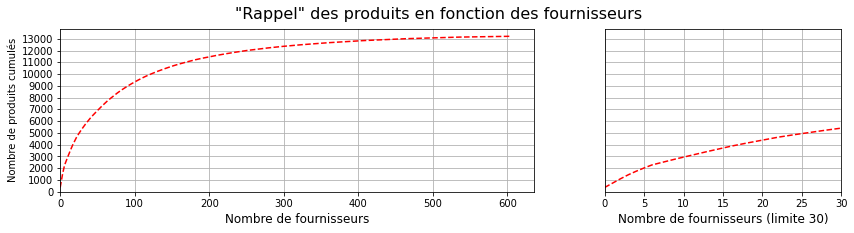
\includegraphics[width=\linewidth]{img/rappel_produit_par_fournisseur.png}
            \end{center}
            \caption{Le Pareto des produits en fonction des fournisseur}
            \label{fig:rappel_pdt_par_frn}
        \end{figure}

        \emphbox{Une approche traditionnelle d'extraction de données depuis des documents pdf ne pourra pas être appliquée pour ce cas d'usage}

        \section{Quelles données ?}

            \subsection{Les principales données et leur mode de présentation dans les fiches techniques}
            Les données que l'on souhaite récupérer sont globalement de 4 types : 
            \begin{itemize}
                \item données de composition : listes d'ingrédients
                \item données de composition : allergènes
                \item données nutritionnelles
                \item données logistiques
            \end{itemize}

            Comme vu dans la section \mref{fiches_techniques}, parmi les données présentes dans les fiches techniques, seule la liste d'ingrédients se présente quasiment toujours sous la forme d'un texte brut (par opposition à un affichage au sein d'un tableau).
            La représentation des données nutritionnelles se fait régulièrement sous forme de tableau, les données logistiques également (cf. les exemples de fiches techniques présentées en annexe, à partir de \mref{ex:FT_sel}).
        
            \subsection{L'identification d'une liste d'ingrédient par son contenu}

            Il est possible de dire si un texte est une liste d'ingrédients, juste en lisant ce texte.
            Il s'agit souvent d'une énumération d'ingrédients individuels (cf. la section \mref{listes_ingredients}).
            Même sortie de son contexte, il est en général faisable pour un humain d'identifier comme telle une liste d'ingrédients.
            Par exemple : 
            \begin{quotation}
                Huile de colza (70.45 \%), jaunes d’oeufs (6.2 \%), purée de tomates, eau, vinaigre, câpres (2.8 \%) (câpres, eau, sel),cornichons (2.8 \%) (cornichons, vinaigre, sel), sucre, sel,amidon modifié, acidifiant : lucono-delta-lactone, conser-vateur : sorbate de potassium, antioxydant : E385 (74mg/kg), épice, arôme naturel aneth
            \end{quotation}
            est de toute évidence une liste d'ingrédients.

            \`{A} l'inverse, les autres grands types d'information nécessitent du contexte dans le document.
            Par exemple, \og 14g \fg peut être une quantité de glucides, de lipides, le poids d'une pièce unitaire, \dots
            
            \emphbox{L'identification de listes d'ingrédients pourrait se faire sans avoir à construire de fonctionnalités s'appuyant sur le contexte au sein du document}

        \section{Quels produits ?}
        
        Pour des raisons d'accessibilité de la donnée, on travaillera sur les produits de la branche \'{E}piSaveurs. 
        Il est de toute façon prévu de déployer le PIM sur l'ensemble des autres branches du groupe, on pourra adresser leurs produits à ce moment-là.
        La notion d'ingrédients n'a pas de sens pour les produits d'hygiène (cf. section \mref{produits_nonal} sur les produits non-alimentaires), mais existe pour les produits de chimie.
        Comme les ingrédients des produits alimentaires sont en général différents des produits de chimie, on se limitera d'abord aux premiers.
        Enfin, la réglementation étant moins stricte pour les boissons alcoolisées sur le sujet spécifique de l'étiquetage de la composition, on ne les prendra pas non plus en compte dans ce mémoire.

        \section{Conclusion quant au choix du cas d'usage}

        \emphbox{Au vu des différentes contraintes listées dans cette partie, on s'attachera à extraire \emph{les listes d'ingrédients} des produits \emph{alimentaires} de la branche \emph{EpiSaveurs} (épicerie et boissons non alcoolisées) depuis \emph{les fiches techniques fournisseur}, en se basant sur \emph{le contenu textuel} de ces documents.}